% Lecture 05 How to write the SRS Sep 2021 Complete: https://docs.google.com/document/d/1fnwYnqAYdEQx13KpmQvulktGNpjKAKfx/edit
% Lecture 05 MSc Project - How to write the SRS Chapter: https://docs.google.com/document/d/1lEheSmKF9sDZkRozLTLSJ8XBDC_4yDxL/edit

% 2. We critically evaluated the Chapter 4 of the sample thesis - https://drive.google.com/drive/folders/1GlPK41lsmaZ26HIwK64AFwvb-3u0Chpx?usp=sharing (Visit Chapter 04 of the thesis and see my comments to see how you can improve)

% --------------

\section{Chapter Overview}
This chapter focuses on identifying possible stakeholders of the project by taking a look at all possible points of interaction with the system with the use of a rich picture diagram, gathering their perceptions to analyse and come up with possible expected use cases, functional and non-functional requirements of the prototype. 

\section{Rich Picture}

% rich picture in canva: https://www.canva.com/design/DAEwtvMqut8/k-BGnDBlelk824WGuNdb7g/edit

\begin{figure}[h!]
\centering
\frame{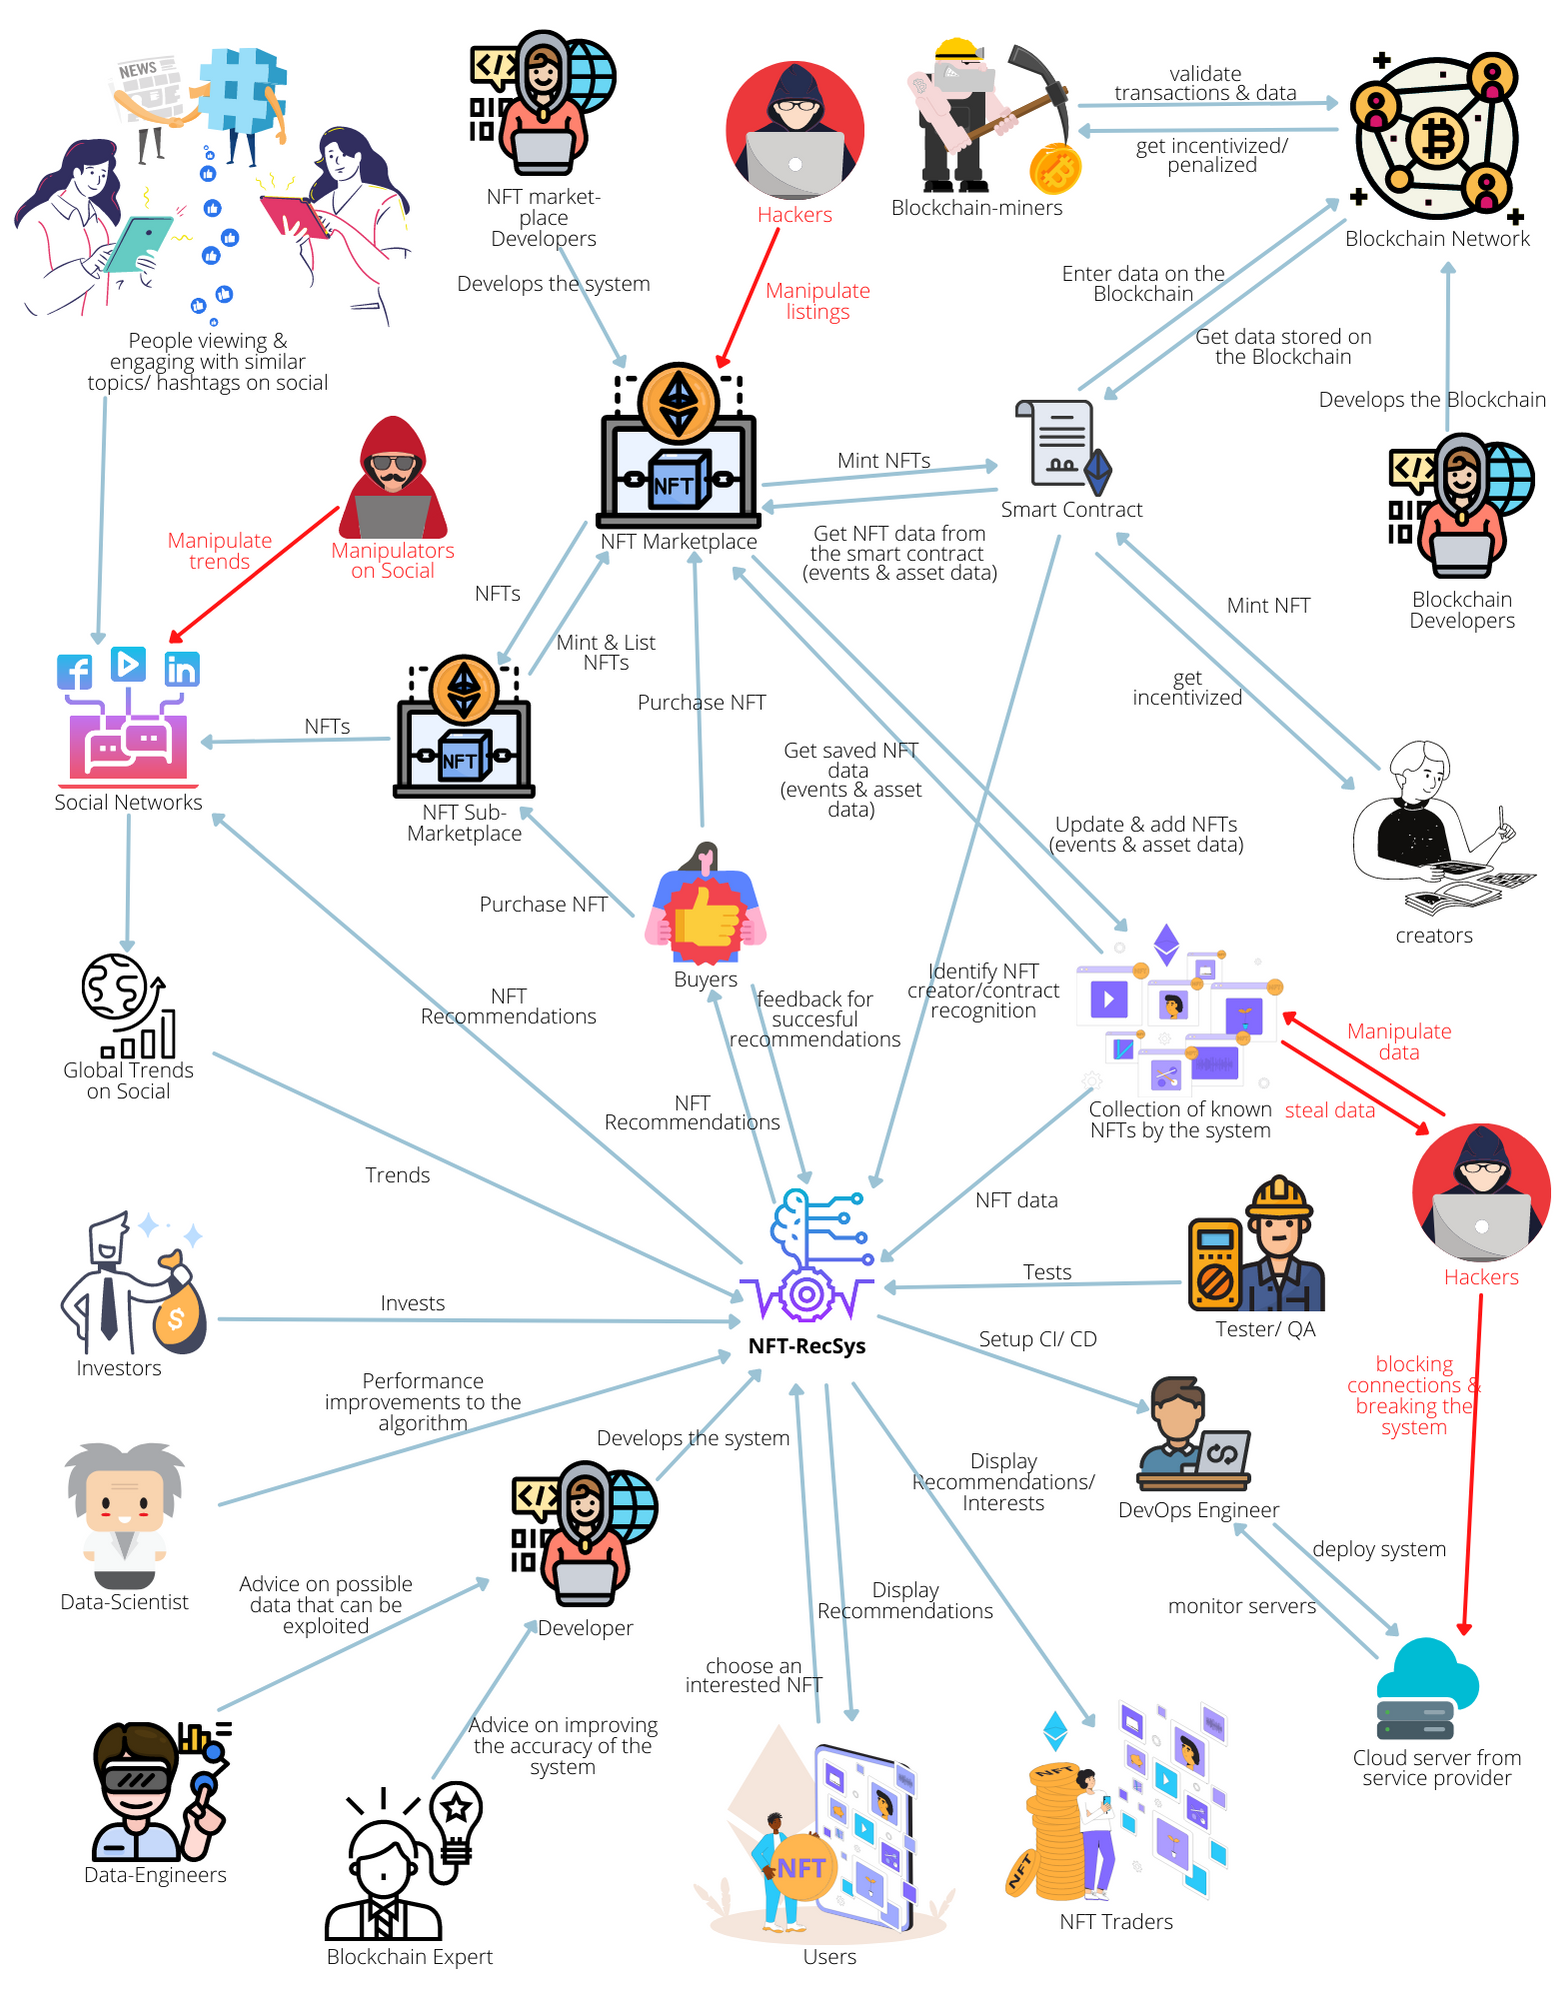
\includegraphics[height=0.65\textheight]{images/SRS/rich-picture.png}}
\caption{Rich Picture Diagram \textit{(self-composed)}}
\label{fig:rich-picture}
\end{figure}

The above Rich Picture diagram shows a helicopter view of how related parties in the rest of the world interacts with the system. It is used to understand the possible interactions that are expected to happen when the system is functional.

\section{Stakeholder Analysis}
The Stakeholder Onion Model illustrates recognized stakeholders who are associated with the system, along with an explanation of each stakeholder's involvement in the system, in Stakeholder Viewpoints.

\subsection{Stakeholder Onion Model}
% figma diagram: https://www.figma.com/file/jEF3LQTiRNXY5tJo6faSDy/FYP---NFT-Recommendation-System?node-id=304%3A3
\begin{figure}[h!]
\centering
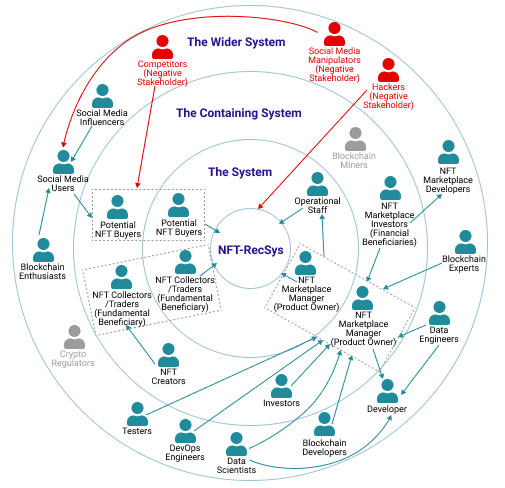
\includegraphics[width=\textwidth]{images/SRS/stakeholder-onion-diagram.png}
\caption{Stakeholder Onion Model \textit{(self-composed)}}
\label{fig:stakeholder-onion}
\end{figure}

\subsection{Stakeholder Viewpoints}
% \usepackage[longtable]{multirow}
% \usepackage{longtable}
% \usepackage{colortbl}


\begin{longtable}{|p{0.25\linewidth}|p{0.27\linewidth}|p{0.4\linewidth}|} 
\caption{Roles and benefits of identified stakeholders}\\ 
\hline
Stakeholder & Role & Benefits/ Role Description \\* 
\hline
Developer & \multirow{2}{*}{Financial Beneficiary} & Creates the system \\* 
\cline{1-1}\cline{3-3}
Investors &  & Makes a profit out of the investments put into marketing, deployments and development of the system \endfirsthead 
\hline
NFT Marketplace Developers & Operational - Maintenance &  \\* 
\hline
Blockchain Experts & \multirow{3}{*}{Expert, Quality Regulator} &  \\* 
\cline{1-1}\cline{3-3}
Data Scientists &  &  \\* 
\cline{1-1}\cline{3-3}
Data Engineers &  &  \\ 
\hline
NFT Creators & Financial Beneficiary &  \\* 
\hline
NFT Traders & \multirow{2}{*}{Fundamental Beneficiary} &  \\* 
\cline{1-1}\cline{3-3}
NFT Collectors, Potential NFT Buyers &  &  \\ 
\hline
NFT Marketplace Manager & System Owner, Operational - Administration &  \\ 
\hline
Operational Staff & Operational - Support &  \\* 
\hline
The Public & \multirow{3}{*}{} &  \\* 
\cline{1-1}\cline{3-3}
Social Media Influencers &  &  \\* 
\cline{1-1}\cline{3-3}
Social Media Users &  &  \\* 
\hline
Hackers & \multirow{3}{*}{Negative Stakeholder} &  \\* 
\cline{1-1}\cline{3-3}
Competitors &  &  \\* 
\cline{1-1}\cline{3-3}
Social Media Manipulators &  &  \\ 
\hline
Blockchain Enthusiasts &  &  \\ 
\hline
Blockchain Miners &  &  \\ 
\hline
Crypto Regulators & Quality Regulator &  \\
\hline
\end{longtable}


\section{Requirement Elicitation Methodologies}

\section{Analysis of Data \& Presentation of the Outcome through Elicitation Methodologies}

% interview & questionnaire questions: https://docs.google.com/document/d/1oNKIeRZbnVcRPimWl0f07go6Uovjzdk5vwATmVQCbFQ/edit

\section{Summary of Findings}

\section{Context Diagram}

\section{Use Case Diagram}

\section{Use Case Descriptions}

\section{Requirements}

\subsection{Functional Requirements}

\subsection{Non-functional Requirements}

\section{Chapter Summary}
In this chapter, a Rich Picture Diagram was drawn to illustrate how the system connects with the society to understand the stakeholders of the system. Saunder's Onion model was used to represent the stakeholders with the flow of influence of each stakeholder. Requirement gathering techniques were utilized to gather all the required data and opinions of possible stakeholders of the system. Lastly, the system's use cases, functional, and non-functional requirements were specified based on the insights derived from the requirement elicitation techniques.